\documentclass[a4paper,14pt]{extarticle}

\usepackage{cmap}
\usepackage[T2A]{fontenc}
\usepackage[utf8x]{inputenc}
\usepackage[english, russian]{babel}

\usepackage{misccorr} % в заголовках появляется точка, но при ссылке на них ее нет
\usepackage{amssymb,amsfonts,amsmath,amsthm}  
\usepackage{indentfirst}
\usepackage[usenames,dvipsnames]{color} 
\usepackage[unicode,hidelinks]{hyperref}
% \hypersetup{%
%     pdfborder = {0 0 0}
% }

\usepackage{makecell,multirow} 
\usepackage{ulem}
\usepackage{graphicx,wrapfig}
\graphicspath{{img/}}
\usepackage{geometry}
\geometry{left=2cm,right=2cm,top=3cm,bottom=3cm,bindingoffset=0cm,headheight=15pt}
\usepackage{fancyhdr} 
\linespread{1.05} 
\frenchspacing 
\renewcommand{\labelenumii}{\theenumii)} 
\newcommand{\mean}[1]{\langle#1\rangle}
% \usepackage{caption}
%%%%%%%%%%%%%%%%%%%%%%%%%%%%%%%%%%%%%%%%%%%%%%%%%%%%%%%%%%%%%%%%%%%%%%%%%%%%%%%
%%%%%%%%%%%%%%%%%%%%%%%%%%%%%%%%%%%%%%%%%%%%%%%%%%%%%%%%%%%%%%%%%%%%%%%%%%%%%%%

\def\labauthors{Сарафанов Ф.Г., Платонова М.В.}
\def\labgroup{430}
% \def\department{Кафедра электроники и квантовой физики}
\def\labnumber{1}
% \def\labtheme{Измерение ширины запрещённой зоны в полупроводниках} 

%%%%%%%%%%%%%%%%%%%%%%%%%%%%%%%%%%%%%%%%%%%%%%%%%%%%%%%%%%%%%%%%%%%%%%%%%%%%%%%
	%применим колонтитул к стилю страницы
\pagestyle{fancy} 
	%очистим "шапку" страницы
\fancyhead{} 
	%слева сверху на четных и справа на нечетных
\fancyhead[L]{\labauthors} 
	%справа сверху на четных и слева на нечетных
% \fancyhead[R]{Отчёт по лабораторной работе №\labnumber} 
\fancyhead[R]{Вынужденная синхронизация} 
	%очистим "подвал" страницы
\fancyfoot{} 
	% номер страницы в нижнем колинтуле в центре
\fancyfoot[C]{\thepage} 
\renewcommand{\phi}{\varphi}
%%%%%%%%%%%%%%%%%%%%%%%%%%%%%%%%%%%%%%%%%%%%%%%%%%%%%%%%%%%%%%%%%%%%%%%%%%%%%%%

\usepackage{float}
\usepackage[mode=buildnew]{standalone}
\usepackage{tikz} 
% \usepackage{subcaption}
\usepackage{tikz,csvsimple}
\usetikzlibrary{scopes}
\usetikzlibrary{%
     decorations.pathreplacing,%
     decorations.pathmorphing,%
    patterns,%
    calc,%
    scopes,%
    arrows,%
    % arrows.spaced,%
}
\makeatletter
\newif\if@gather@prefix 
\preto\place@tag@gather{% 
  \if@gather@prefix\iftagsleft@ 
    \kern-\gdisplaywidth@ 
    \rlap{\gather@prefix}% 
    \kern\gdisplaywidth@ 
  \fi\fi 
} 
\appto\place@tag@gather{% 
  \if@gather@prefix\iftagsleft@\else 
    \kern-\displaywidth 
    \rlap{\gather@prefix}% 
    \kern\displaywidth 
  \fi\fi 
  \global\@gather@prefixfalse 
} 
\preto\place@tag{% 
  \if@gather@prefix\iftagsleft@ 
    \kern-\gdisplaywidth@ 
    \rlap{\gather@prefix}% 
    \kern\displaywidth@ 
  \fi\fi 
} 
\appto\place@tag{% 
  \if@gather@prefix\iftagsleft@\else 
    \kern-\displaywidth 
    \rlap{\gather@prefix}% 
    \kern\displaywidth 
  \fi\fi 
  \global\@gather@prefixfalse 
} 
\newcommand*{\beforetext}[1]{% 
  \ifmeasuring@\else
  \gdef\gather@prefix{#1}% 
  \global\@gather@prefixtrue 
  \fi
} 
\makeatother

\usepackage{booktabs}
\usepackage{pgfplots, pgfplotstable}

\usepackage[outline]{contour}
\usepackage{tocloft}
\renewcommand{\cftsecleader}{\cftdotfill{\cftdotsep}} % for parts
% \renewcommand{\cftchapleader}{\cftdotfill{\cftdotsep}} % for chapters
\usepackage{pgfplots,pgfplotstable,booktabs,colortbl}
\pgfplotsset{compat=newest}
\usepackage{physics}
\usepackage{cancel}
\usepackage{mathtools}
\mathtoolsset{showonlyrefs=true}
\newcommand\Smat{\hat { \mathbf { S } }}

\newcommand*\dotvec[1][1,1]{\crossproducttemp#1\relax}
\def\crossproducttemp#1,#2\relax{{\qty[\vec{#1}\times\vec{#2}\,]}}

\newcommand*\prodvec[1][1,1]{\crossproducttempa#1\relax}
\def\crossproducttempa#1,#2\relax{{\qty[{#1}\times{#2}\,]}}

% \def\E{\mathscr{E}_H}
\def\Rdim{\,\frac{\text{м}^3}{\text{А} \cdot \text{с}}}

\renewcommand{\vec}{\mathbf} % for parts

\begin{document}
\begin{titlepage}
\begin{center}
% \vspace{-3em}
{\small\textsc{Нижегородский государственный университет имени Н.\,И. Лобачевского}}
\vskip 2pt \hrule \vskip 3pt
{\small\textsc{Радиофизический факультет}}

\vfill


{{\large Отчет по лабораторной работе №\labnumber}\vskip 12pt {\Huge \bfseries Вынужденная \\[10pt] синхронизация}}

	
\vspace{2cm}
{\large Работу выполнили студенты \\[-0.25em] 430 группы радиофизического факультета \\[0.5em] {\Large \bfseries \labauthors}}

% \vspace{0.5cm}
% {e-mail: sfg180@yandex.ru}

% \vspace{2cm}

\end{center}

\vfill
	
% \begin{flushright}
% 	{Выполнили студенты 430 группы\\ \labauthor}%\vskip 12pt Принял:\\ Менсов С.\,Н.}
% \end{flushright}
	
% \vfill
	
\begin{center}
	{Нижний Новгород, 23 апреля -- \today}
\end{center}

\end{titlepage}
\tableofcontents
\newpage




% \end{document}

\section*{Введение}
\addcontentsline{toc}{section}{Введение}

В данной работе изучается явление \textit{вынужденной синхронизации}  автогенератора под воздействием внешней гармонической силы с частотой $\omega$, достаточно близкой к его собственной частоте $\omega_0$. При этом можно наблюдать явление \textit{захвата частоты}: в определенном диапазоне расстройки $\omega-\omega_0$ и амплитуды внешней силы $\rho$ автогенератор совершал колебания на частоте внешнего воздействия.

\section{Мягкий режим возбуждения}
\subsection{Модель генератора и анализ в мягком режиме}
Для простого лампового генератора с гармоническим воздействием уравнения, описывающие его динамику, при пренебрежении сеточным током (его можно сделать малым) будут следующими \cite{orlov,matrosov}:
\begin{equation}
	\label{eq:1}
	L\dv{i}{t}+Ri+u=M\dv{i_a(u)}{t}+E_0+E\cos \omega t, \qquad
	i=C\dv{u}{t}+\xcancel{i_c(u)}
\end{equation} 
Нелинейность $i_a(u)$ аппроксимируется полиномом третей или пятой степени. При этом третья степень всегда дает мягкий режим возбуждения колебаний, в отличии от пятой. В реальном генераторе выбор режима обуславливается напряжением смещения $E_0$. В данной работе будут использованы и мягкий, и жесткий режим возбуждения.

В мягком режиме анодно-сеточная характеристика лампы имеет вид
\begin{equation}
	i(u)=i_0+S_0u-\gamma u^3
\end{equation}
Причем рабочая точка выбрана так, что $S(u_0)=0$ и отсюда $\gamma=S_0/(3u_0^2)$. Введем новые безразмерные переменные:
\begin{gather}
	\omega_0^2=\frac{1}{LC},\quad
	\mu=\frac{\omega_0^2\qty(MS_0-RC)}{\omega}, \quad
	\varepsilon_0=\frac{E\omega_0^2}{u_0\omega^2}\sqrt\frac{MS_0}{MS_0-RC},\\
	x=\frac{u}{u_0}\sqrt\frac{MS_0}{MS_0-RC}, \quad
	\varepsilon=\frac{\varepsilon}{\mu}, \quad
	\xi=\frac{\omega^2-\omega^2_0}{\mu \omega^2}, \quad \tau_1=\mu \omega t, \tau=\mu\tau_1
\end{gather}
Здесь $\varepsilon$ -- амплитуда внешнего воздействия, $\xi$ -- относительная расстройка частот, а $\mu, \varepsilon_0 \ll 1$ -- малые параметры. В этих переменных уравнение \eqref{eq:1} перепишется в виде
\begin{equation}
	\ddot{x}+x=\mu \qty[\qty(1-x^2)\dot{x}+\varepsilon\cos\tau+\xi x], \qq{где} \mu \ll 1
\end{equation}
Из этого уравнения можно методом Ван-дер-Поля получить систему автономных укороченных уравнений \cite{nkrkn}:
\begin{gather}\left\{
	\begin{aligned}
		\dot{\rho}&=\rho\qty(1-\rho^2)+\varepsilon \sin\phi\\
		\dot{\phi}&=-\xi+\frac{\varepsilon}{\rho} \cos\phi
	\end{aligned}\right.
\end{gather}
Из системы можно выразить биквадратное уравнение резонансных кривых, отвечающих состоянию равновесия укороченной системы (а значит, периодическим движениям исходной системы):
\begin{equation}
	\rho^2(1-\rho^2)^2+\xi^2\rho^2=\varepsilon^2
\end{equation}
Несложный анализ состояний равновесия даст разбиение на области устойчивости резонансных кривых \cite{matrosov}.

\subsection{Экспериментальные результаты}
\subsubsection{Резонансные кривые}
\begin{figure}[h!]
	\centering
	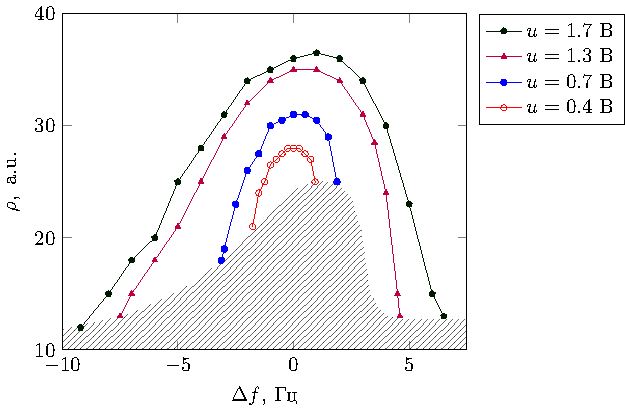
\includegraphics[width=0.9\textwidth]{plot/test}
	\vspace{-1em}
	\caption{Экспериментальные кривые в мягком режиме}
	\label{fig:figure1}
\end{figure}

% * разделить слабые и сильные сигналы (как переходят: скачком или нет)

Мы подобрали напряжение смещения так, чтобы автогенератор работал в мягком режиме. При этом частота автогенератора составила $f_0=424.67$ кГц, а амплитуда колебаний $\rho = 25$ a.u. 

Затем мы подали внешнее воздействие, и изменяя частоту внешнего воздействия $f$, сняли зависимость амплитуды колебаний автогенератора от частоты $f$. График же был построен от расстройки $\Delta f=f-f_0$.

Штрихованная область на графике отвечает окончанию синхронизации и переходу в режим биений. Это неустойчивая область резонансных кривых, она появилась, как и предсказывает анализ состояний равновесия укороченной системы.

В случае напряжений $u=0.4$ В, $u=0.7$ В реализовался сценарий рождения колебаний  скачком, и их можно классифицировать как \textit{слабые сигналы}. При напряжениях $u=1.3$ В, $u=1.7$ В колебания при изменении расстройки рождались мягко, и следовательно, это -- \textit{сильные сигналы}.

\subsubsection{Ширина полосы захвата и удержания}

Мы обозначили следующим образом (см. рис. \ref{fig:band}, стр. \pageref{fig:band}) частоты, при которых наблюдается гистерезис на границе полосы синхронизации и провели измерения этих частот в диапазоне амплитуд внешнего воздействия $u=0.5\ldots 1.5$ В.
\begin{figure}[h!]
	\centering
	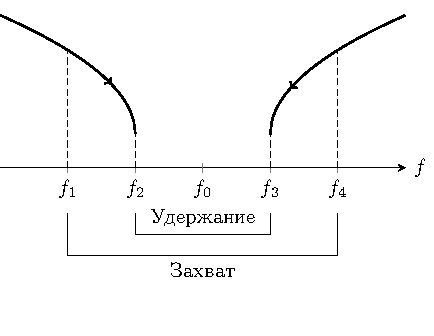
\includegraphics[scale=1.5]{fig/band.pdf}
	\vspace{-2em}
	\caption{Обозначение частот при гистерезисе}
	\label{fig:band}
\end{figure}
По полученным результатом мы построили графики зависимости полосы удержания синхронизации и полосы захвата синхронизации от амплитуды внешнего воздействия (см. рис. \ref{fig:band2}, стр. \pageref{fig:band2}).
\begin{figure}[H]
	\centering
	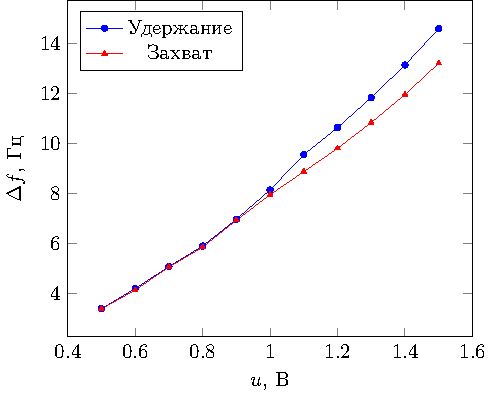
\includegraphics[width=0.7\textwidth]{plot/band.pdf}
	\vspace{-1em}
	\caption{Экспериментальные результаты полос синхронизации}
	\label{fig:band2}
\end{figure}
\begin{figure}[H]
	\centering
	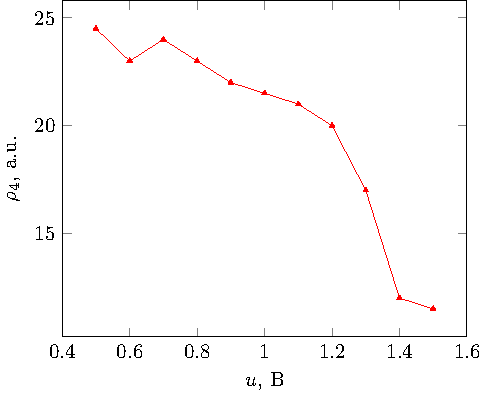
\includegraphics[width=0.7\textwidth]{plot/ampl.pdf}
	\vspace{-1em}
	\caption{Экспериментальная зависимость амплитуды на границе}
	\label{fig:ampl}
\end{figure}
% \clearpage
% \newpage
\subsubsection{Амплитуда на правой границе полосы синхронизации}
Мы провели эксперимент по определению амплитуды колебаний автогенератора на границе полосы удержания синхронизации (по введенным обозначениям -- на частоте $f_4$), и построили полученную зависимость (см. рис. \ref{fig:ampl}, стр. \pageref{fig:ampl}).

% \newpage
\section{Жёсткий режим возбуждения}
\subsection{Экспериментальные результаты}
\subsubsection{Резонансные кривые}
\begin{figure}[H]
	\centering
	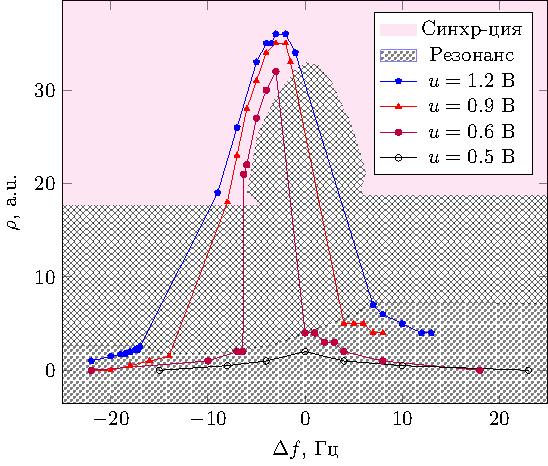
\includegraphics[width=0.8\textwidth]{plot/hard.pdf}
	\vspace{-1em}
	\caption{Резонансные кривые в жёстком режиме (эксперимент)}
	\label{fig:hard}
\end{figure}
\subsubsection{Биения в окрестности синхронизации}
\begin{figure}[H]
	\centering
	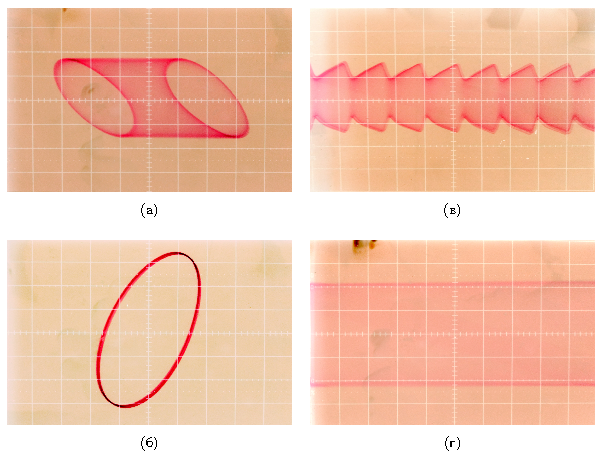
\includegraphics[width=\textwidth]{plot/photo.pdf}
	\vspace{-2em}
	\caption{Фигура Лиссажу и осциллограмма в режиме биений (а), (в),  в режиме синхронизации (б), (г)}
	\label{fig:liss}
\end{figure}


\begin{figure}[H]
	\centering
	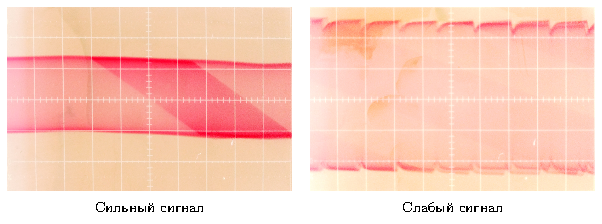
\includegraphics[width=\textwidth]{plot/level.pdf}
	\vspace{-2em}
	\caption{Осциллограммы режима биений в окрестности синхронизации}
	\label{fig:bie}
\end{figure}

\newpage
\addcontentsline{toc}{section}{Список литературы}
\begin{thebibliography}{99}

\bibitem{orlov} Орлов И.\,Я., Односевцев В.\,А. и др. Основы радиоэлектроники: учебное пособие. -- Нижний Новгород: Нижегородский государственный университет им. Н.И. Лобачевского, 2011. -- 169 с.

\bibitem{matrosov} Матросов В.\,В. Вынужденная синхронизация:  учебно-методическое пособие. -- Нижний Новгород: Нижегородский государственный университет им. Н.И. Лобачевского, 2013. -- 40 с.

\bibitem{nkrkn}  Некоркин В.\,И. Лекции по основам теории колебаний: учебное пособие. -- Нижний Новгород: Нижегородский государственный университет им. Н.И. Лобачевского, 2011. -- 233 с.  

% \bibitem{sh}    Шалимова К.В. Физика полупроводников. М.: 1982.
\end{thebibliography}
\end{document}